\documentclass[twocolumn]{article}
\usepackage{graphicx}
\usepackage{algorithm}
\usepackage{verbatim}
\newcommand{\kmer}{$k$-mer}
\newcommand{\kmers}{$k$-mers}
\newcommand{\dna}[1]{\hbox{\small \texttt{\uppercase{#1}}}}

\begin{document}

\section{Introduction}

Short read sequencing platforms (e.g. Illumina) have become a high quality source of sequence
data in a short space of time.  It is now routine to get tens or
hundreds of millions of reads from a sequencing run: reads of length
100bp, and with an error rate of below 1\%. Furthermore, these
errors are overwhelmingly dominated by substitution errors, which
tend to be easier to deal with than insertions and deletions (indels).
This high accuracy is unfortunately offest by the relatively short
read length.

Conversely, newer single molecule sequencing platforms (e.g. Pacific Biosciences)
yield long reads --- thousands to tens of thousands of base pairs, however the
error rates are significantly higher (10\%--15\%),
and are dominated by insertions and deletions.
The length of the reads makes them very attractive, but the error rate makes using them difficult.

It is appealing to use a mix of short and long read data to get the benefits for both.
\cite{xxx} have done this, using short read data to correct the long reads. However,
their method has two important limitations. Their method is slow; and it reports only corrected
regions of reads, and can therefore discard some of the long range structural information which
makes long reads attractive.
This method works by aligning the short reads on to the long ones.

We propose an alternative method for correcting the long reads. Using our existing assembly methods
for short reads \cite{goss2012}, we use de Bruijn graph assembly methods to remove errors from the
short read data. We can then align the long reads to the de Bruijn graph, using the fact that each
long read should correspond to a path in the de Bruijn graph. The errors in the long read will mean
that a combination of error correction and search will be required to identify the correct
correspondence.

\section{Methods}

\begin{figure}
\begin{center}
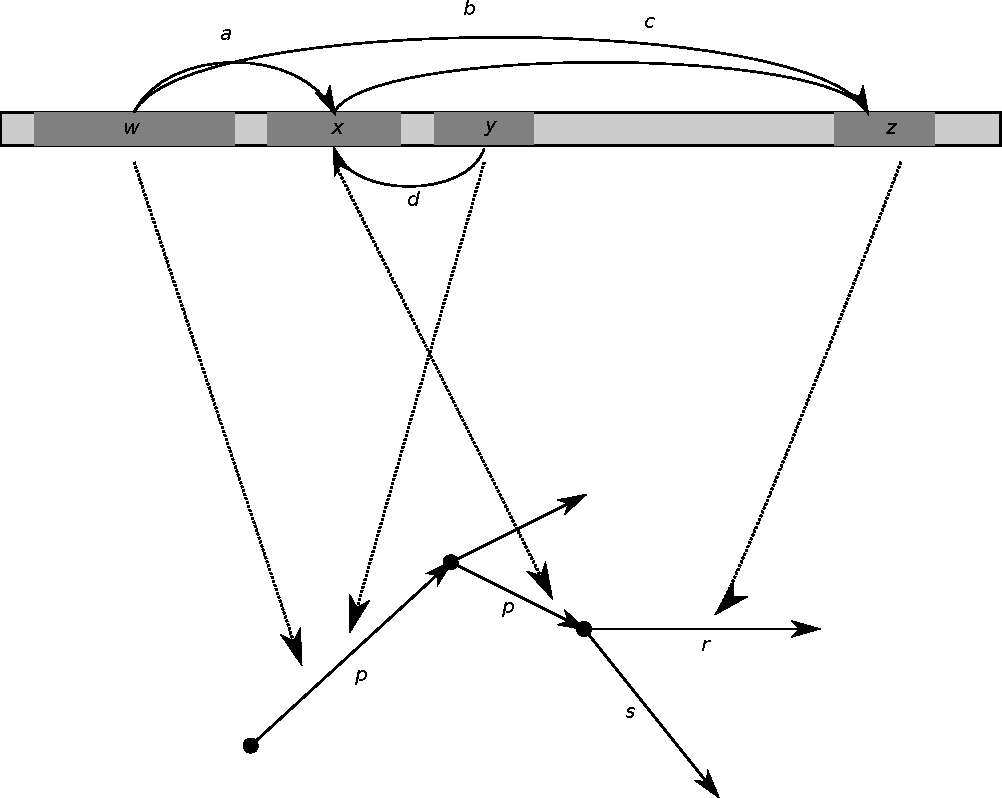
\includegraphics[scale=0.5]{scheme.pdf}
\end{center}
\caption{
This figure gives a schematic representation of how the error
correction process takes place.  In the read, depicted as the gray
rectangle in the top of the figure, there are four seeds labeled
\textsl{w} -- \textsl{z}. A piece of the de Bruijn graph is depicted
in the bottom part of the figure, with segments labeled \textsl{p}
-- \textsl{s}.  The arcs \textsl{a} -- \textsl{d} denote hypothesized
correspondences between the read and the graph.  Arc \textsl{a} is
identified by our algorithm because the seeds \textsl{w} and
\textsl{x} map into adjacent segments \textsl{p} and \textsl{q} of
the graph. Likewise, \textsl{c} is also identified. Arc \textsl{b}
is not, though could be if we expended extra computational effort
to search beyond adjacent segments.  Arc \textsl{d} is rejected
because the path in the graph is in the wrong direction. The graph
is symmetric over reverse complementation so we can ignore such
inconsistent arcs.  The weight of an arc, such as \textsl{a} is
determined by the length of the seeds \textsl{w} and \textsl{x}
(longer seeds being less likely to be spurious), and the coherence
between the distance between \textsl{w} and \textsl{x} in the read
and their distance in the graph.
}
\label{fig:uniqueness}
\end{figure}

\begin{figure}
\label{fig:algo}
\begin{verbatim}
R is a sequence of long reads
S is a set of short reads

1. construct de Bruijn graph G from S
     perform spectral error removal on G
     perform structural error removal on G

   for each r in R:
2.   identify candidate seeds
3.   form a graph connecting
       mutually consistent seeds
4.   choose connected components
5.   paste corroborated segments
6.   align to extend into gaps
\end{verbatim}
\caption{A high level sketch of the long read correction algorithm.}
\end{figure}

Our method for error correcting the long reads is conceptually very
simple: construct the de Bruijn graph of the underlying genome with
the short reads, then align the long reads to the de Bruijn graph.
This is outlned in Figure~\ref{fig:algo}.
The principle difficulties lie in the fact that the long reads have
a high indel rate, making it difficult to identify true seeds; there
are places where the short read coverage drops to zero, so there
are breaks in the path; and there are \textit{tangles} in the de
Bruijn graph where there are many alternative brancing and cyclic
paths, which make it computationally expensive to identify a matching path.

The method takes one or more files of short reads and one or more
files containing long reads as input and outputs files corresponding
to the long read files with the corrected parts of the reads in
upper case and the parts of the read that could not be corrected
(because of ambiguity in the graph or holes in the coverage of the
short read data).  By keeping the long reads intact in this way,
we retain the information present in them about the relationship
between the corrected parts.

\subsection{De Bruijn Graph Construction}
\label{sec:cons}

The first phase of the algorithm, constructing the de Bruijn graph from the short reads,
yields a representation of the underlying genomic sequence with very few residual errors,
and because the representation we use is self-indexing, it allows for efficient alignments.
The construction algorithm is the same as used for assembly, as described in \cite{goss2012}.
The de Bruijn graph $k_g$, with a value of 32 being typical, which we denote specially
because we will use \kmers\ with various $k \le k_g$ in later phases of the algorithm.
What we have at the point where we leave the assembly process is a de Bruijn graph
represented as a set of edges. Sequences of edges that form non-branching paths in
the graph are called \textit{linear segments}. Linear segments may be uniquely identified
by their first edge, and we construct an index which allows us to take an arbitary edge
and identify its containing linear segment and the offset of the edge within the segment.
We also have an index that allows us to find the length of each linear segment.

The second and subsequent phases of the algorithm are performed on each long read.

\subsection{Identifying Seeds}
\label{sec:seeds}

The second phase is finding seed \kmers\ in a long read for performing local
alignment to the de Bruijn graph from those seeds by following paths in the graph.

The de Bruijn graph $\mathbf{G}$ is represented as a set of \kmers\ which are accessed through the
\textit{rank}/\textit{select} API due to \cite{Jacobson89}. In brief, the API supports
the following two fundamental operations, given a set of integers (called \textit{positions})
from a domain $[0,n)$:
\begin{description}
\item[$\textit{rank}(p)$] is the number of integers in the set that are strictly less than $p$
\item[$\textit{select}(r)$] is the $r^\textit{th}$ smallest element of the set
\end{description}

From these two operations we can derive several useful operations.
$$
    \textit{access}(p) = \textit{rank}(p + 1) - \textit{rank}(p)
$$
which has the value 1 if $p$ is in the set, and 0 if it is not.
This may be generalized to \textit{count}:
$$
    \textit{count}(p_1, p_2) = \textit{rank}(p_2) - \textit{rank}(p_1)
$$
which tells yields the number of elements in the half-open interval $[p_1, p_2)$.

Noting that an edge in the de Bruijn graph may be interpreted as an integer with
$2k$ bits\footnote{assuming $\texttt{A} = 0$, $\texttt{C} = 1$, and so on},
we can trivially scan a long read and invoke \textit{access} with $k_g$-mers to locate seeds for the subsequent
parts of the alignment algorithm. However, as noted, because of the error charactersitics of the long
reads, the probability of finding an error free $k_g$-mer is very unlikely. However, using \textit{count}
we can scan for shorter \kmers\ very efficiently. For $k \le k_g$, we can evaluate:
$$
    \textit{access}_k(x) = \textit{count}(x \times 4^d, (x+1) \times 4^d)
$$
where $d = k_g - k$. That is, we count the number of $k_g$-mers that have the \kmer\ $x$ as a prefix.

For each position $i$ in the long read we can find the longest seed \kmer\ $x_i$ for which
$\textit{access}_k(x_i) = 1$.
The value of $k$ at position $i$ is $k_i$.
We filter the putative seeds in several stages to remove seeds that are likely to be spurious and lead to false alignments.

Given $k_i$, we require that $k_{i+1} \ge k_i$ since if $k_{i+1}$ were less than $k_i$,
such the seed $x_{i+1}$ would give no information not already implied by the seed $x_i$.
If $k_{i+1} < k_i$, it is dropped as a candidate seed.

Our basic confidence $s_i$ that a seed $x_i$ is not spurious is measured by the probability that an arbitary $k_i$-mer
will be observed in the de Bruijn graph $\mathbf{G}$.
That is
$$
    s_i = \left\{
        \begin{array}{ll}
            1 - \frac{\left|G\right|}{4^{k_i}}  & \textrm{if } \left|G\right| \le 4^{k_i} \\
            0                                   & \textrm{if } \left|G\right| > 4^{k_i}
        \end{array}
          \right.
$$

That puts a lower bound on $k_i$:
$$
k_i \ge \lceil \log_4 \left|G\right| \rceil
$$

\subsection{Connecting Seeds}
\label{sec:graph}

The main technique for detecting groups of seeds that are likely to lead to accurate alignments
is to form a directed graph with a node for each candidate seed and joining pairs of seeds with weighted
edges where the weight reflects a confidence that the distance between the seeds in the read is consistent
with their distance in the de Bruijn graph, according to a statistical error model.

We construct a directed graph with a seed $x_i$ at each node, and
an edge with weight $w_{ij}$ between each pair of nodes
$\left<x_i,x_j\right>$ such that $i < j$.  The weight on each edge
reflects our confidence that the pair of seeds are not spurious and
that the distance $j - i$ between them in the read is consistent
with the distance between $x_i$ and $x_j$ in the de Bruijn graph.
Edges with a weight of 0 are dropped from the graph.

To compute our confidence $d_{ij}$ that the distance between
$x_i$ and $x_j$ in the graph is consistent with their distance in the read
(i.e. $j - i$) we use a model that assumes an independent probability of a
single base insertion or deletion at each position is $p$.
(Our model may trivially be generalized to account for distinct rates
for insertions and deletions, but we do not do so here for brevity.)
By looking up the \kmers\ in the graph, we can locate the linear segment
from which they came, and their offset within the containing segment. If
$x_i$ and $x_j$ are in the same linear segment of the de Bruijn graph,
then their displacement
may be computed trivially. We can search in the de Bruijn graph very
cheaply to see if the linear segment of $x_j$ is an immediate successor
of the linear segment of $x_i$. If so, again, the displacement may be
trivially computed. 
It would be possible do deeper searching in the de Bruijn graph to locate
a path connecting the two seeds, but such search quickly becomes very expensive,
and the possibility of locating spurious paths increases.

The computed distance we denote $l_{ij}$ If by these
means we cannot compute the displacement in the de Bruijn graph, then 
no corresponding edge is placed in the directed graph.
We can model the insertions and deletions independently
as binomial processes, and arrive at a multinomial model, however,
since for our scoring function we will be only interested in the central
region around the mean, we can approximate with a normal distribution
using the variance of the binomial distributions $l_{ij}p(1-p)$.
Thus we compute $d_{ij}$:
$$
    d_{ij} = \mathcal{N}\left(0, 2l_{ij}p\left(1 - p\right), X \ge \left|l_{ij} - \left(j - i\right)\right|\right)
$$
And:
$$
    w_{ij} = s_i s_j d_{ij}
$$

We discard any edge with $w_{ij} < w_{\textit{min}}$.

\subsection{Extracting Mutually Consistent Seeds}
\label{sec:comp}

Having constructed a graph describing hypothesized homology between
the long read and the de Bruijn graph, the next stage of the algorithm
is to determine which nodes and edges form the most likely set of consistent
information, and discard those parts of the graph that are inconsistent.

Each connected component denotes the alignment of a segment of the long read to
the de Bruijn graph. We consider each connected component in turn, ordered by the
component with the greatest cumulative edge weight, most weighted component first.

For each component we consider whether its span on the long read is consistent with
previously considered components. If it is not, it is discarded.

\subsection{Pasting Sequences from the de Bruijn Graph}
\label{sec:paste}

For each component, we follow a path from the left-most seed following
the most heavily weighted edge amongst choices. This yields a span
in the read and a sequence of linear segments. The sequence between
the left-most and right-most seeds in the path can simply be pasted
in to the read.

Various other heuristic algorithms could be used to identify spans of the
de Bruijn graph that can simply be pasted in to the corrected long read,
but we find that this simple algorithm is fast, accurate and robust.

\subsection{Perform Alignment to Fill Gaps}
\label{sec:gaps}

The pasting process may leave gaps where the preceeding the left-most
seed of a component or following the right-most seed of a component.
It is frequently the case that these seeds map into the interior
of a linear segment in the de Bruijn graph, and therefore we can
extend the corrected sequence unambiguously to the end of the linear
segment. To identify the point in the long read that corresponds
to the end of the linear segment we use the Needleman-Wunsch algorithm
\cite{Needleman}. We note that because we only need the length of
the optimal alignment, this can be done in linear space.
Having obtained the length of the optimal alignment, we can again
paste the corresponding sequence from the de Bruijn graph in to the
long read.

The result is a read in which parts have been corrected/corroborated by
the de Bruijn graph and parts may be uncorrected/uncorroborated. These
are denoted in the output by upper and lower case respectively.

\section{Results}

\section{Discussion}

There are many points in the algorithm where we have made simple heuristic algorithmic choices,
including the following.
\begin{itemize}
\item When searching for seeds, we restrict candedates to cases where $\textrm{access}_k = 1$. If cases
where $\textrm{access}_k > 1$ were allowed, some potential alignments may be discovered. It would lead to
more nodes and edges in the directed graph.
\item When determining the distance between seeds in the de Bruijn graph, we restrict the search to seeds
in the same or adjacent linear segments. Deeper search would discover more paths.
\item When determining which paths in the de Bruijn graph to paste in to a long read, a very simple heuristic
treatment of the directed graph is used. A more subtle treatment might lead to slightly more of the read being
corrected.
\end{itemize}

In all cases, these choices take simple constant time algorithms
and turn them in to depth first or similar search algorithms which
tend to be expensive. In most cases, while they may result in more
true-positive opportunities for correcting parts of long reads, in
many cases they are likely to result in much higher liklihood of
fasle-positives, resulting in miscorrection.

\end{document}
